%%%%%%%%%%%%%%%%%%%%%%%%%%%%%%%%%%%%%
%% MORTALITY VS. ED RANK SCATTERPLOTS
%%%%%%%%%%%%%%%%%%%%%%%%%%%%%%%%%%%%%
\begin{landscape}
\begin{figure}[htbp]
  \floatpagestyle{empty}
  \caption{Mortality vs. Education Rank, Age 50--54,
    1992--1994 to 2016--2018}
  \label{fig:mort_scatters}
  \begin{center}
    \begin{tabular}{cc}
    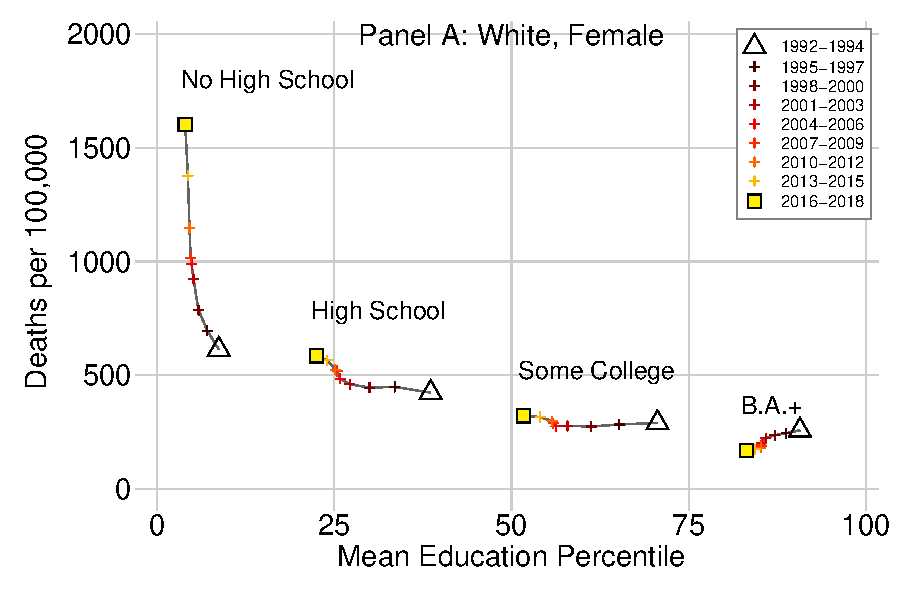
\includegraphics[scale=.6]{\mortalitypath/scatter-smooth-t-50-2-1}
    & 
    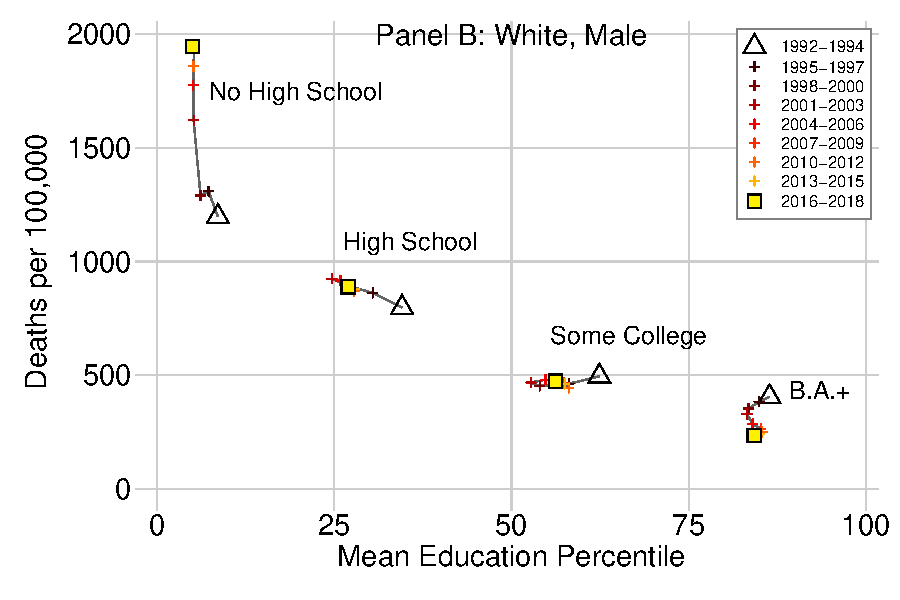
\includegraphics[scale=.6]{\mortalitypath/scatter-smooth-t-50-1-1}
    \\
    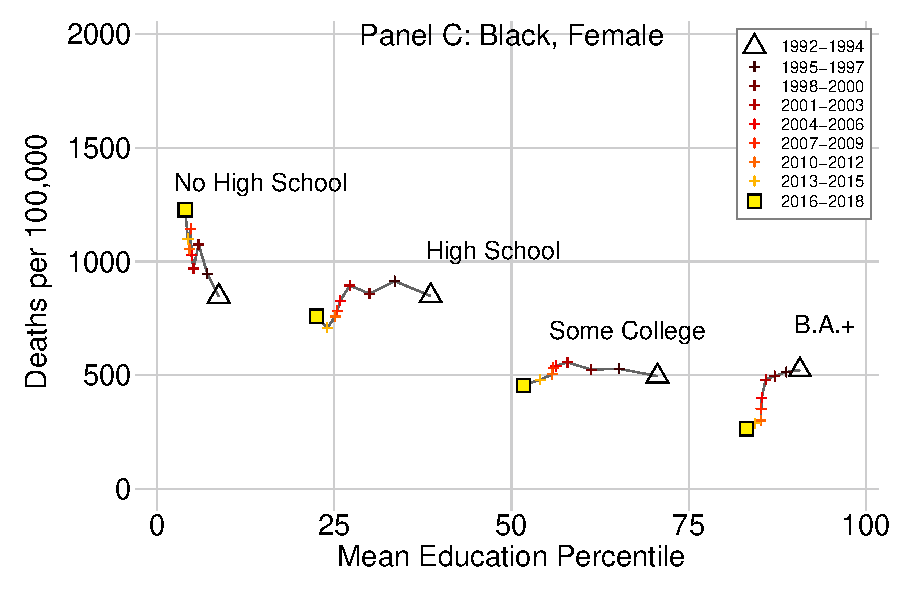
\includegraphics[scale=.6]{\mortalitypath/scatter-smooth-t-50-2-2}
    & 
    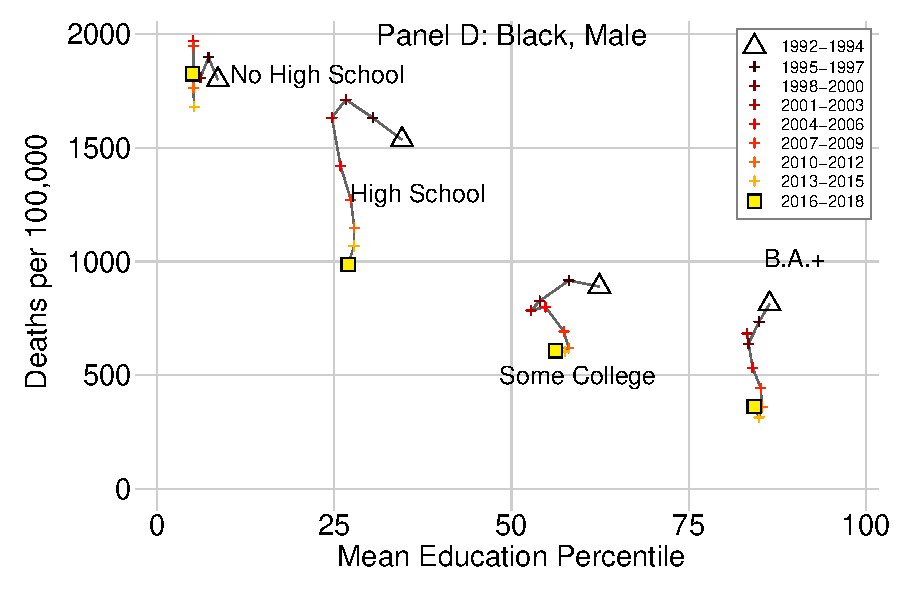
\includegraphics[scale=.6]{\mortalitypath/scatter-smooth-t-50-1-2}
    \end{tabular}
  \end{center}
    \footnotesize{Note: ``White'' refers to non-Hispanic white and
      ``Black'' to non-Hispanic black. The figure shows change in
      mortality and average education rank for individuals aged 50--54
      at different levels of education, from 1992--1994 to 2016--2018. Each point
      represents the average number of deaths per 100,000 people among
      people with one of four levels of education: No High School,
      High School, Some College, and a B.A. or Higher. The $X$
      coordinate of each point represents the average education
      percentile among people with the given level of educational
      completion. For example, a 50-year-old white woman with a high school
      education was at the 39th percentile of the education
      distribution in 1992--1994 and at the 22nd percentile in
      2016--2018. Sources: ACS, CPS, NCHS.}
\end{figure}
\end{landscape}

%%%%%%%%%%%%%%%%%%%%%%%%%%%%%%%%%%%%%
%% INTUITIVE MU-BOUNDS EXPLANATION %%
%%%%%%%%%%%%%%%%%%%%%%%%%%%%%%%%%%%%%
\begin{figure}[H]
\thispagestyle{empty} 
  \caption{Calculating the CEF of Mortality Given Education Rank}
  \label{fig:intuit}
  \begin{center}
    \begin{tabular}{c}
      
      \panel{Panel A ($\mu_0^{10}$): Observe that $\mu_0^8$ is point identified and $\mu_8^{10}$ is bounded between 535 and 800} \\
      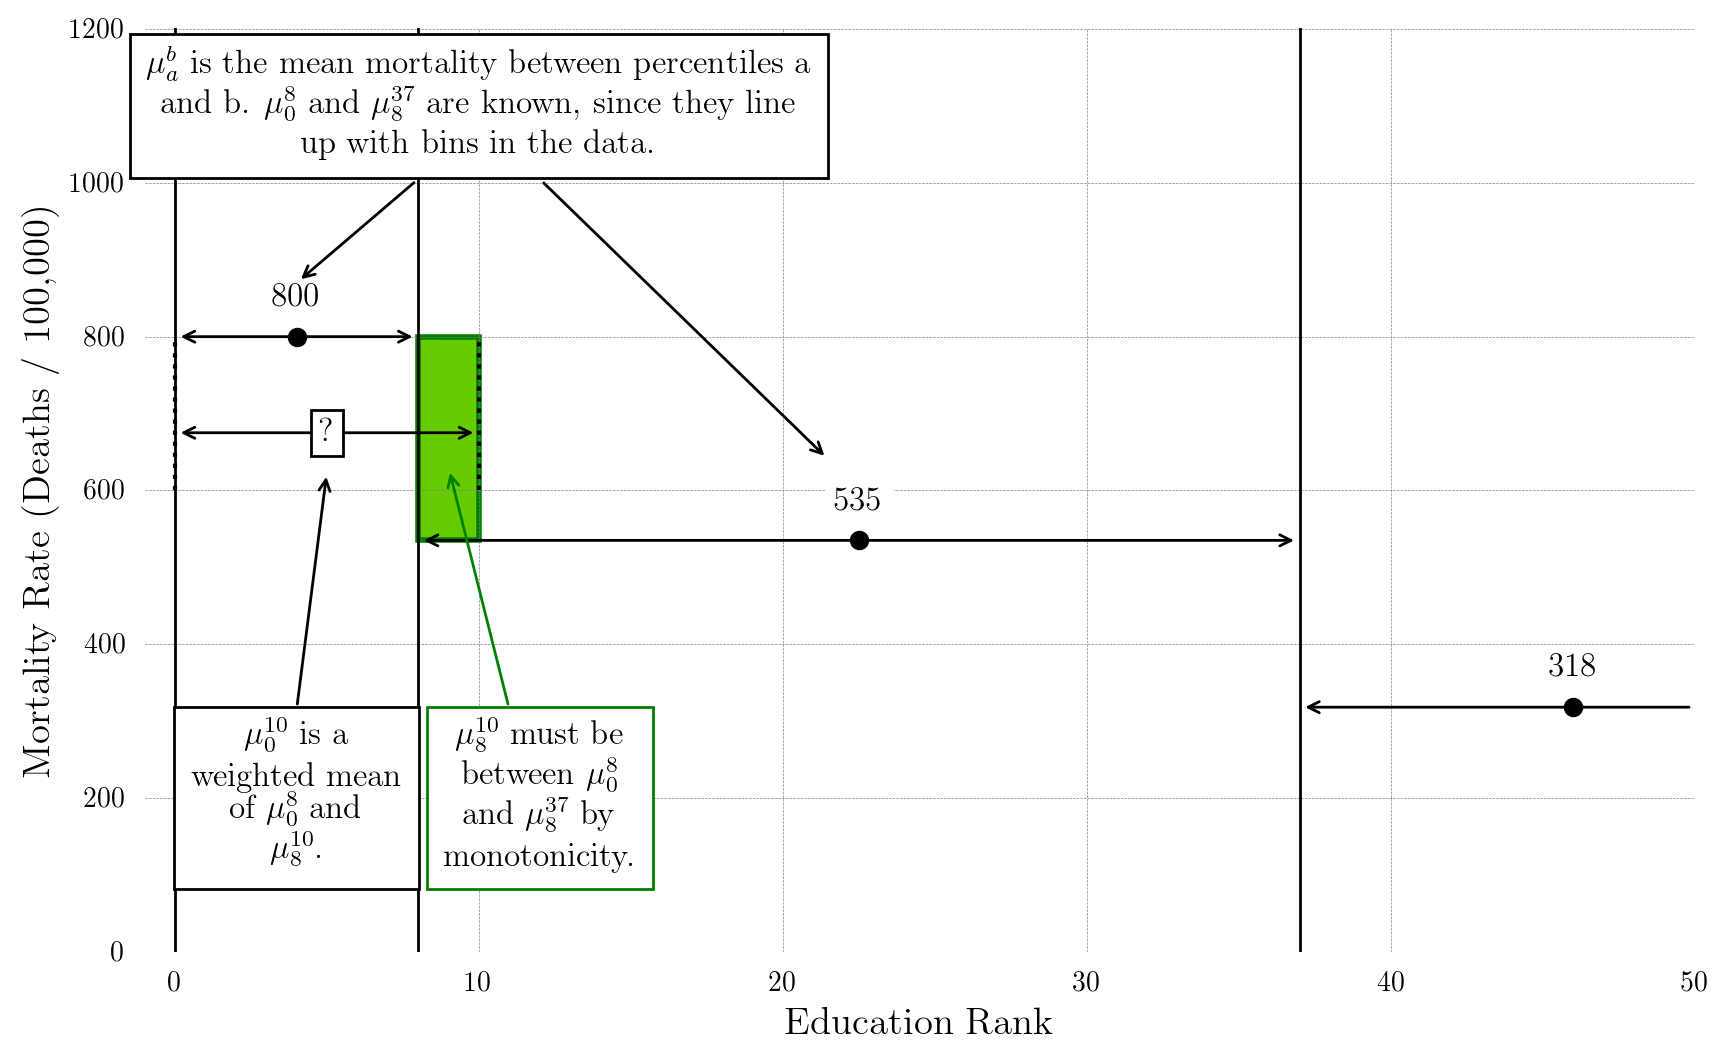
\includegraphics[scale=0.75]{\mortalitypath/intuit_a} \\
      
      \panel{Panel B ($\mu_0^{10}$): Obtain bounds by averaging $\mu_0^8$ and $\mu_8^{10}$} \\
      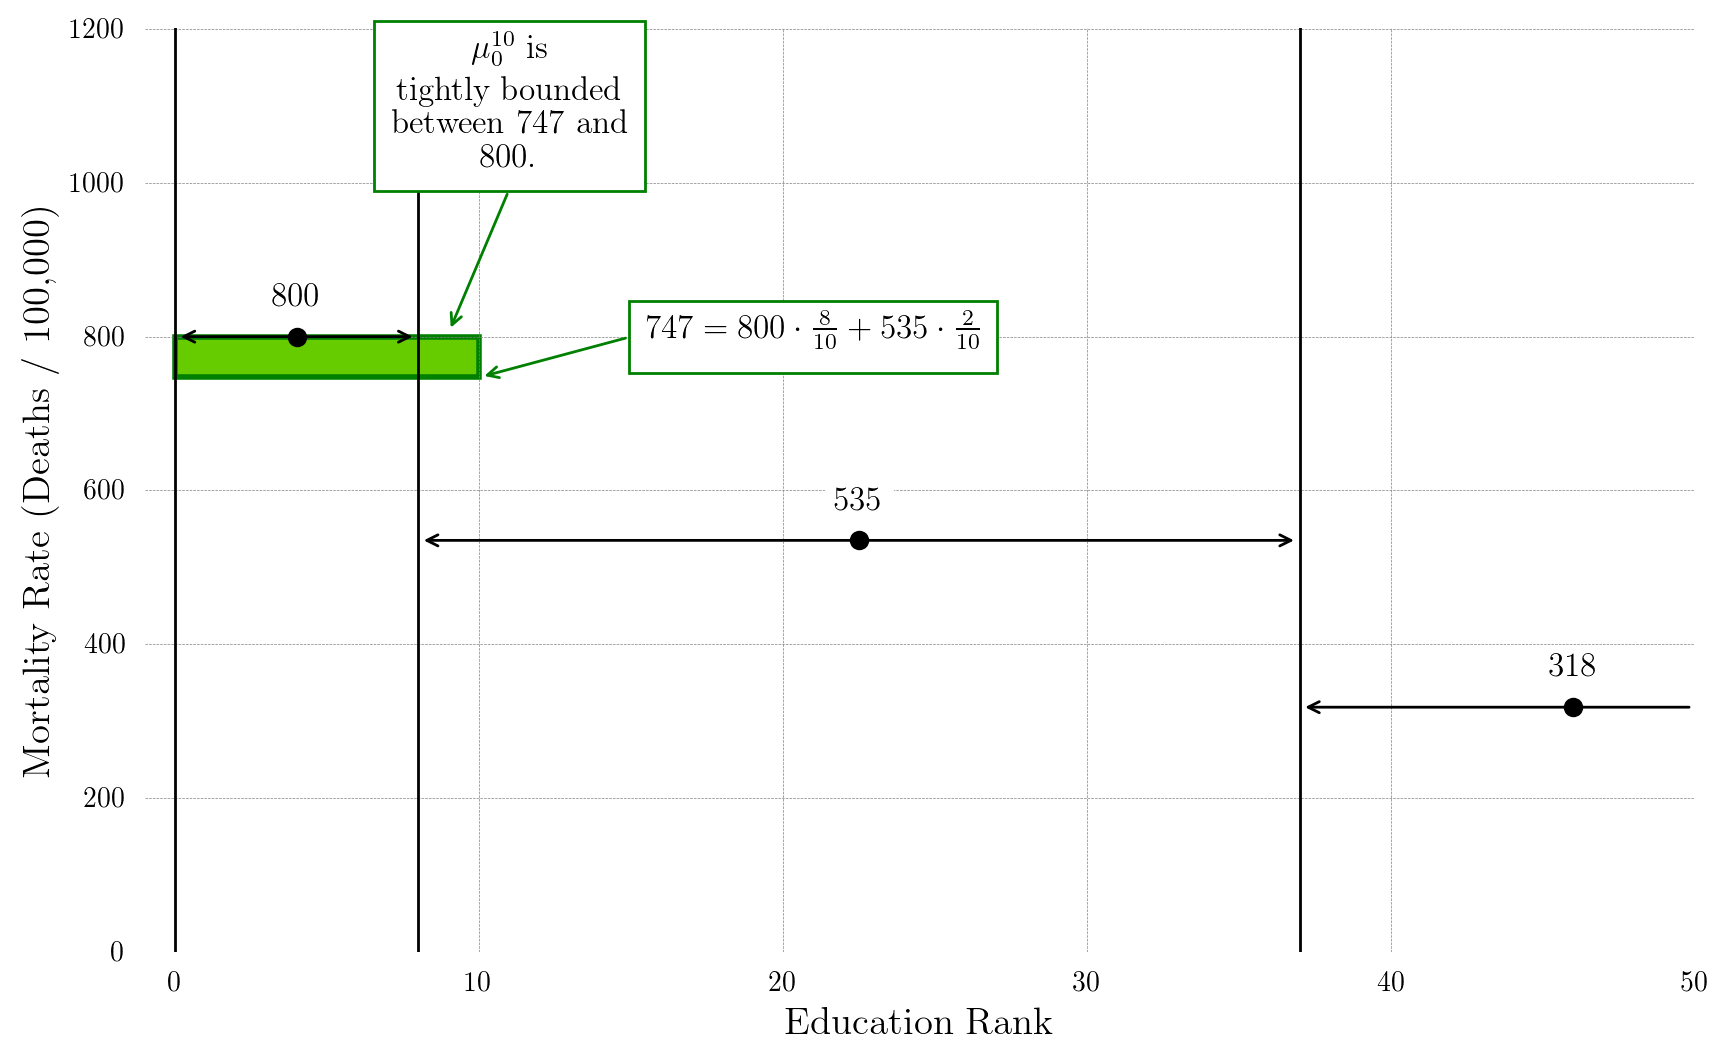
\includegraphics[scale=0.75]{\mortalitypath/intuit_b} \\
      
    \end{tabular}
  \end{center}
\end{figure}

\begin{figure}[H]\ContinuedFloat
\thispagestyle{empty} 
  \begin{center}
    \begin{tabular}{c}

      \panel{Panel C ($\mu_{10}^{40}$): Obtain the lowest possible value of $\mu_{10}^{37}$ ($=$ 515)} \\
      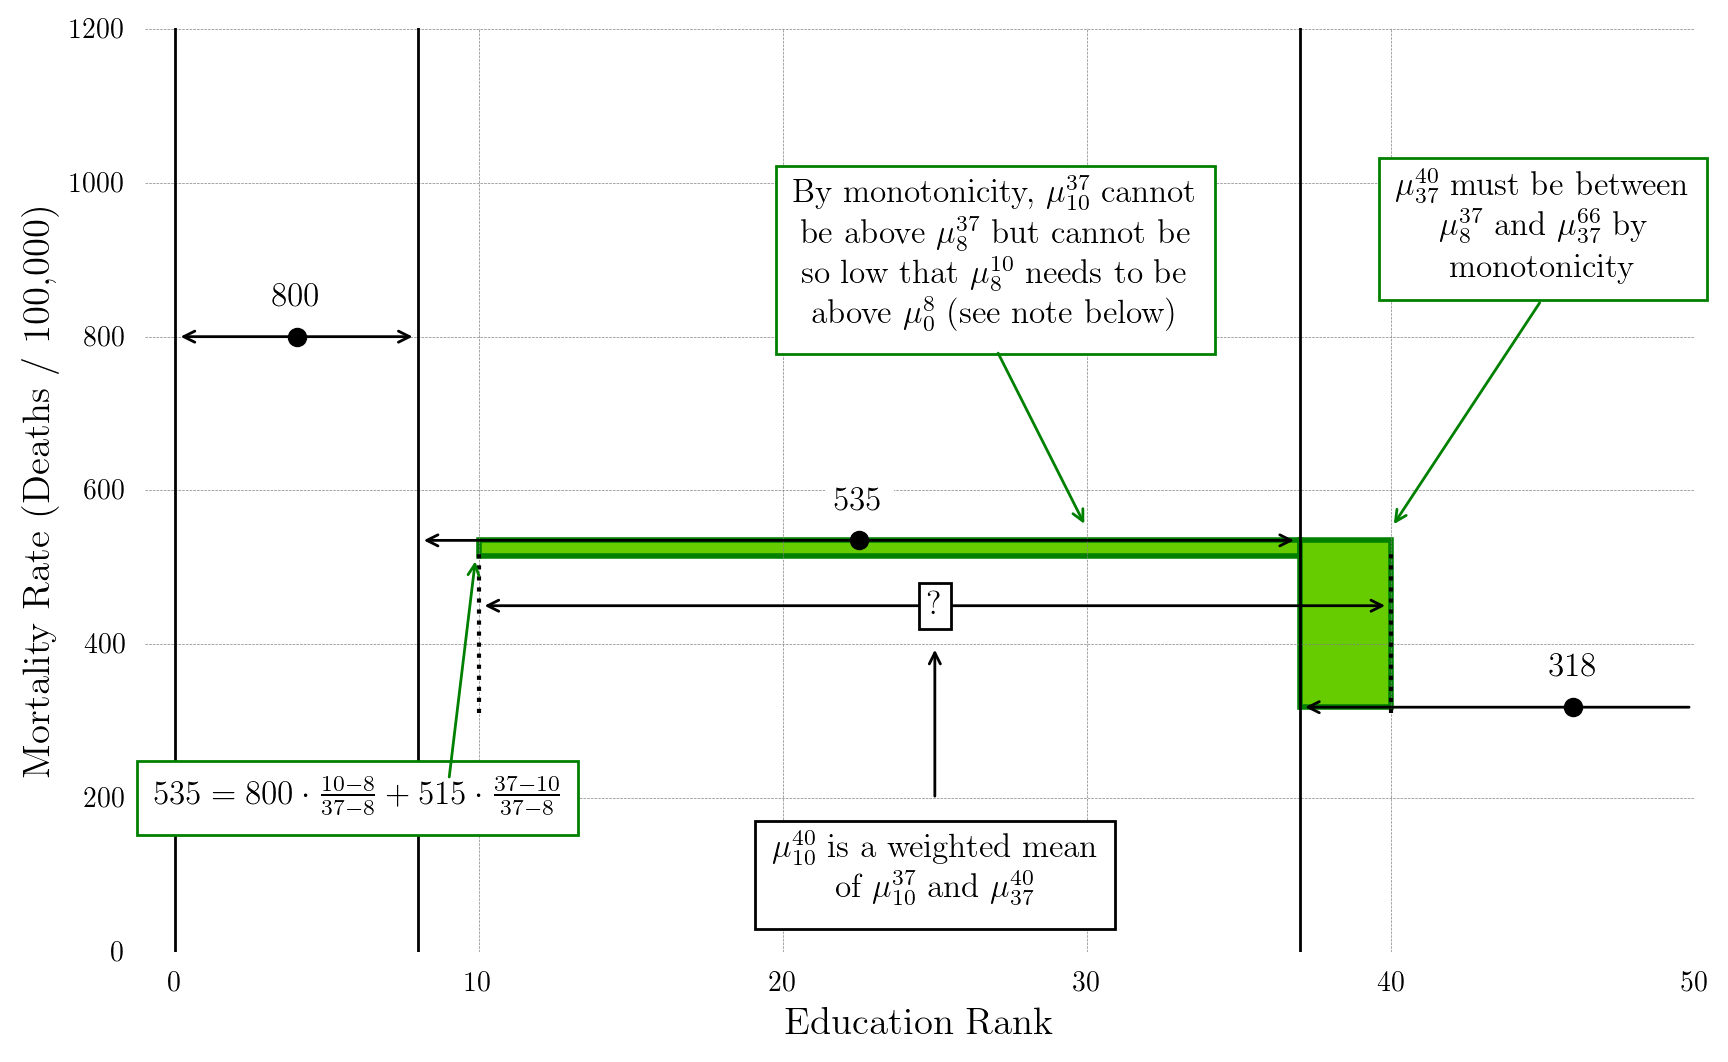
\includegraphics[scale=0.75]{\mortalitypath/intuit_c} \\
      
      \panel{Panel D: ($\mu_{10}^{40}$): Using the lowest value of $\mu_{10}^{37}$, average with the lowest value of $\mu_{37}^{40}$ ($=$318)} \\
      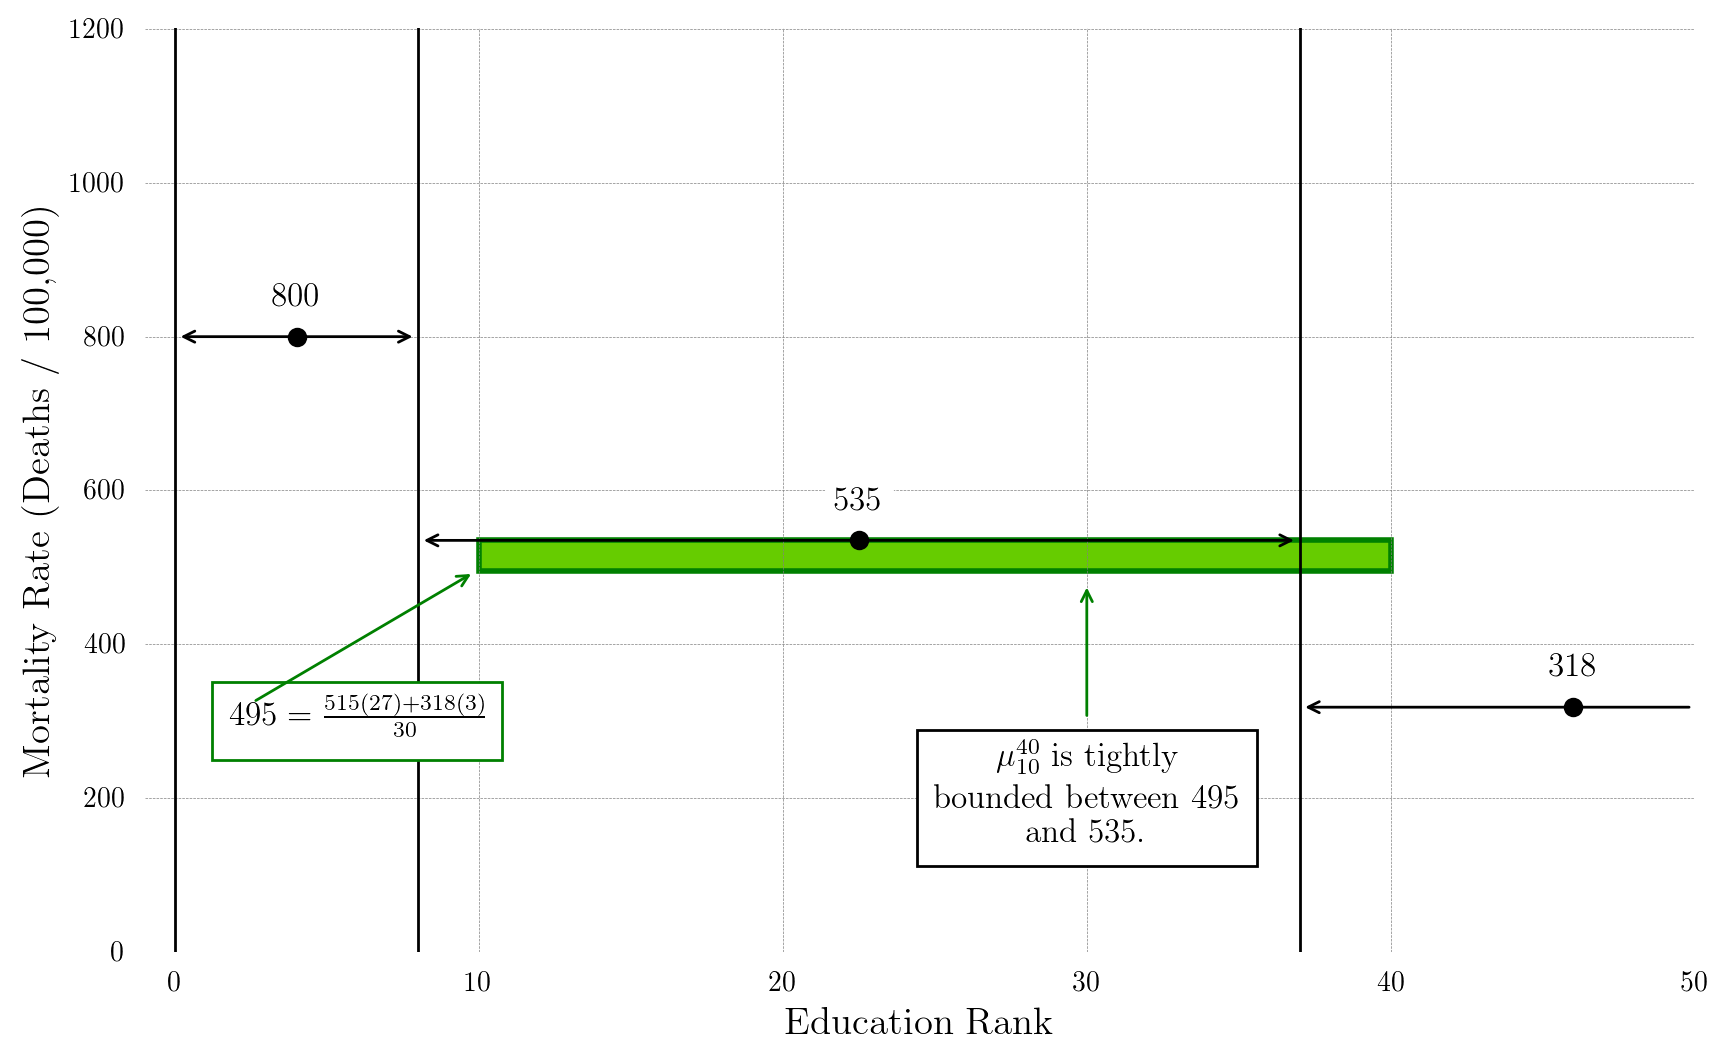
\includegraphics[scale=0.75]{\mortalitypath/intuit_d} \\
      \hline
    
    \end{tabular}
  \end{center}
  \noindent
  \footnotesize{Figure \ref{fig:intuit} provides a graphical description of the calculation of the bounds on $\mu_a^b$ in two scenarios. The data are from women aged 50--54 in 2016--18. The vertical lines show the rank bin boundaries for each education bin for this group. The points show the mean mortality in each bin. The first two panels show the calculation of $\mu_0^{10}$ and the following two panels show the calculation of $\mu_{10}^{40}$. In Panel C, the upper bound of $\mu_{10}^{37}$ cannot exceed the value of $\mu_8^{37}$, because that would require $\mu_8^{10} > \mu_{10}^{37}$. The lower bound cannot be below 515, or else $\mu_8^{10}$ would need to be higher than $\mu_0^8$ to fit the bin mean, thus violating monotonicity. Source: NCHS.}
\end{figure}

%%%%%%%%%%%%%%%%%%%%%%%%%%%
%% MORTALITY CEF COMPARE %%
%%%%%%%%%%%%%%%%%%%%%%%%%%%
\begin{figure}[H]
\caption{Change in Total Mortality of U.S. Women, Age 50--54
  \cnewline Bounds on Conditional Expectation Functions}
\label{fig:mort_overlay}
\begin{center}
    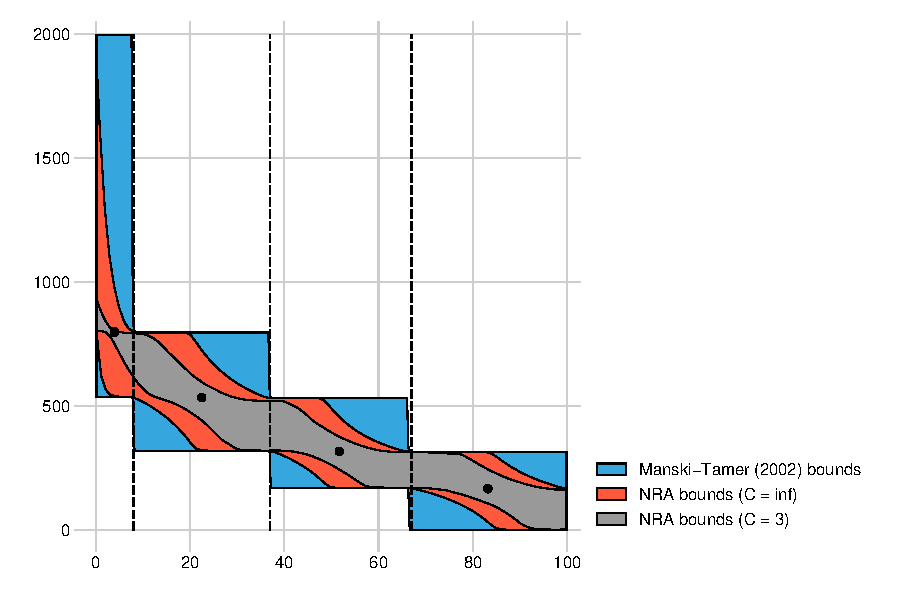
\includegraphics[scale=1.1]{\mortalitypath/mort_cef}
\end{center}
\noindent
\footnotesize{Figure \ref{fig:mort_overlay} shows bounds on the
  conditional expectation function of mortality as a function of
  latent educational rank. The sample consists of U.S. women aged
  50--54; mortality is measured in deaths per 100,000 women. The
  points in the graph show the mean education rank and mortality in
  each year for individuals with (i) less than high school; (ii) high
  school; (iii) some college; and (iv) a B.A. or higher. The curves
  show the bounds on expected mortality at each latent parent rank
  ($E(Y|X=i)$ in the text). The outer (blue) bounds are calculated
  following \cite{Manski2002}. In the bottom bin, the blue bounds are
  truncated at 2,000 for visual clarity but actually extend to 100,000
  (since the procedure cannot reject a mortality rate of 1 up to the
  first bin cut). The middle (red) bounds are calculated following our method with unrestricted curvature. The tightest (gray) bounds are calculated restricting the curvature to 3\% of mean mortality across every percentile bin (2x the largest curvature found in U.S. income rank-rank data \citep{Chetty2016b}.). Education rank is measured relative to the set of all women aged 50--54. Source: NCHS}

\end{figure}
 
%%%%%%%%%%%%%%%%%%%%%%%%%%%%%%%%%%%%%%%%
%% BIAS OF MORTALITY CHANGE ESTIMATES %%
%%%%%%%%%%%%%%%%%%%%%%%%%%%%%%%%%%%%%%%%
\begin{figure}[htbp]
\caption{Changes in U.S. Mortality, Age 50--54, 1992--94 to 2016--18:
  \cnewline Naive and Constant Rank Interval Estimates (Women, Ages 50--54)}
\label{fig:mort_bias}
\begin{center}

  \begin{tabular}{c}
    Panel A: Less than High School \\
    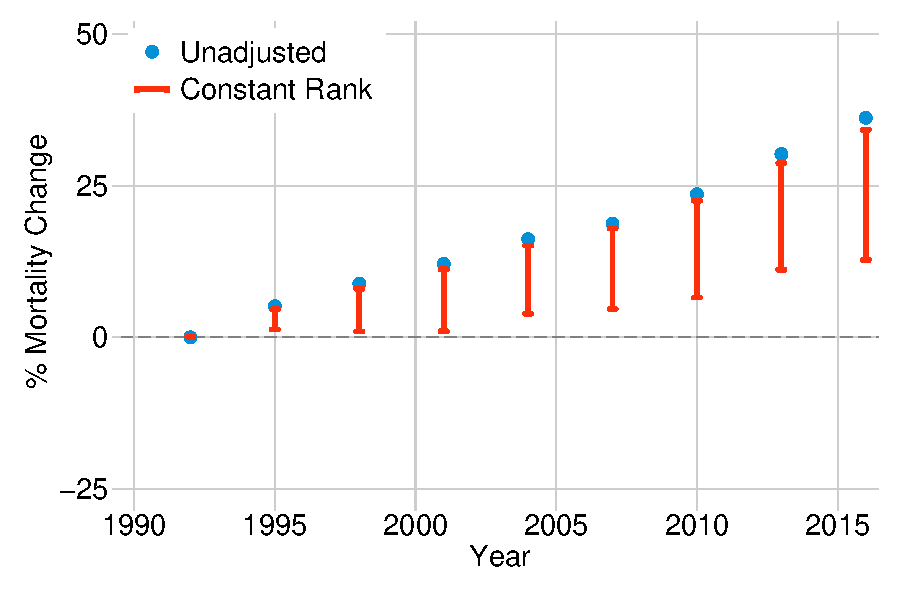
\includegraphics[scale=.8]{\mortalitypath/naive-5-women-50-t-1}
    \\
 Panel B: High School \\
    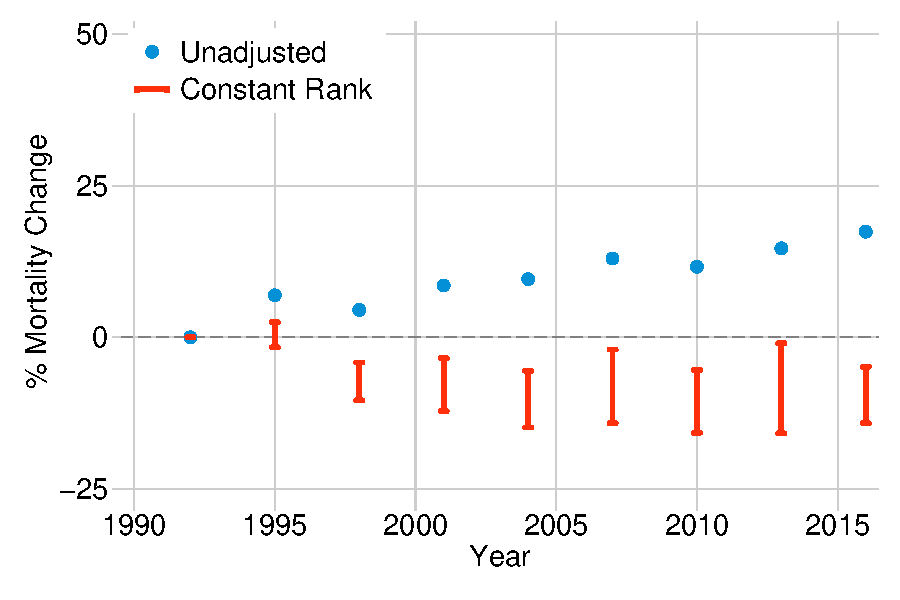
\includegraphics[scale=.8]{\mortalitypath/naive-5-women-50-t-2} \\
    \hline
  \end{tabular}
\end{center}
\noindent
Figure~\ref{fig:mort_bias} shows mortality changes for 50--54-year-old women from 1992--94 to 2016--18 (all races combined), calculated under different methods. The points show unadjusted estimates for women at constant education levels---dropouts in Panel A and high school graduates in Panel B. Both of these population groups have shrunk as proportions of the population during the sample period. The vertical bars show bounds on mortality change in constant rank bins---ranks 0--17 in Panel A and ranks 17--60 in Panel B. These ranks are chosen because they are close to the share of women in 1992--1994 with less than a high-school degree or exactly a high school degree, allowing the bounds to be very tight in the starting period.
\end{figure}

%%%%%%%%%%%%%%%%%%%%%%%%%%%%%%%%%%%%%
%% BOUNDED MORTALITY TRENDS BY GROUP
%%%%%%%%%%%%%%%%%%%%%%%%%%%%%%%%%%%%%
\begin{figure}[H]
  \floatpagestyle{empty}
    \caption{All-Cause Mortality Change in Constant Education
      Percentiles: \cnewline Age 50--54, 1992--1994 to 2016--2018}
    \label{fig:trend}
    \begin{center}
      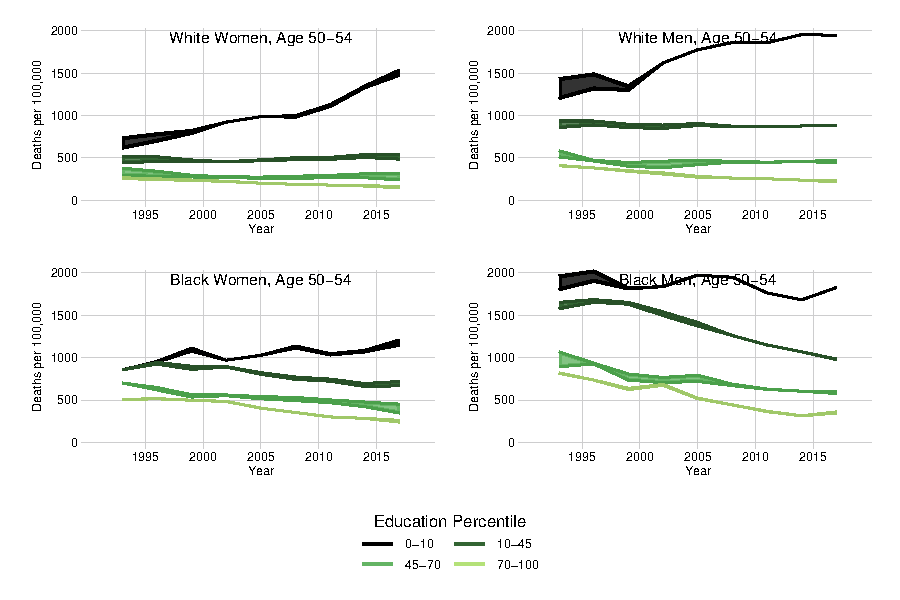
\includegraphics[scale=1.1]{\mortalitypath/trend-smooth-mon-step-t-sex-50}
    \end{center}
  \footnotesize{Note: ``White'' refers to non-Hispanic white and ``Black'' to non-Hispanic black.  Each interval represents the bounded set containing the number of deaths per 100,000 people in a given time period, among people in the education percentiles specified in the legend. The education percentiles correspond to the percentile bins describing four levels of education for the median age group in 2003: No High School, High School, Some College, and a B.A. or Higher. Bounds are computed as described in Section~\ref{sec:method}. The sample consists of people ages 50--54. Sources: ACS, CPS, NCHS.}
\end{figure}

%%%%%%%%%%%%%%%%%%%%%%%%%%%%%%%%%%%%%%%%%%%%%%%%%%%%%%%%%%%%%%%%
% Figure:      Main Mortality Estimates                        %
%              White Women, White Men, Black Women, Black Men  %
%%%%%%%%%%%%%%%%%%%%%%%%%%%%%%%%%%%%%%%%%%%%%%%%%%%%%%%%%%%%%%%%

\begin{figure}[H]
  \floatpagestyle{empty}
  \caption{Mortality Change in Constant Education
    Percentiles (1992--1994 to 2016--2018, All Ages)}
  \label{fig:mort_main}
  \begin{center}
    \begin{tabular}{c}
      \panel{\textbf{A. Non-Hispanic White Women}} \\
      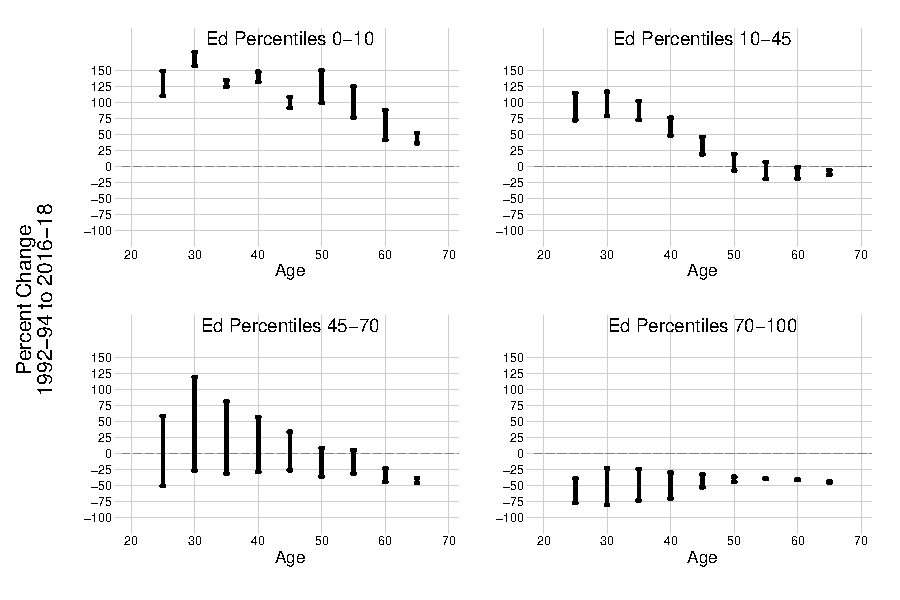
\includegraphics[scale=0.9]{\mortalitypath/changes-total-2-1} \\
      \panel{\textbf{B. Non-Hispanic White Men}} \\
      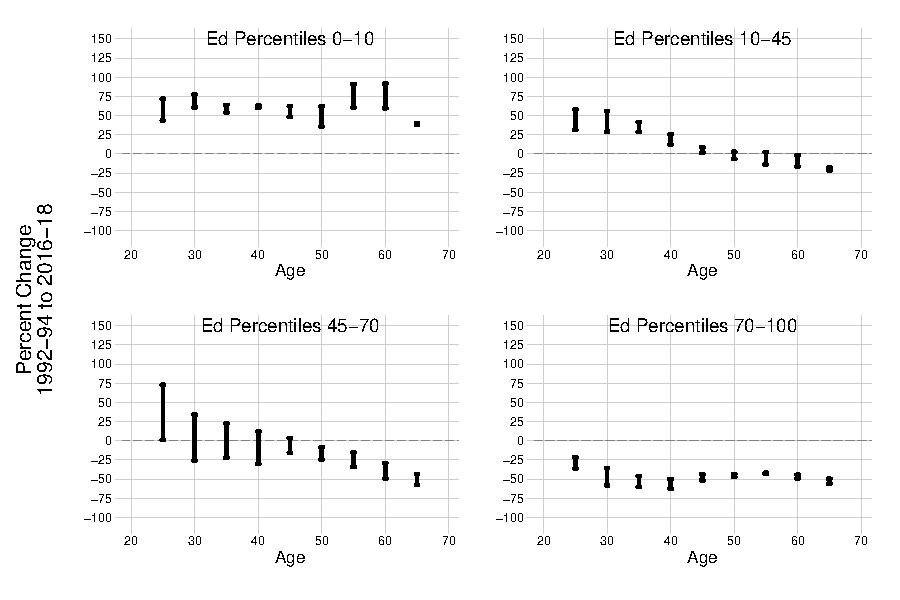
\includegraphics[scale=0.9]{\mortalitypath/changes-total-1-1} \\
    \end{tabular}
  \end{center}
  \vspace{-.5cm} \scriptsize{The graph shows changes in mortality by age, sex, race, and
    constant percentile education bin. The vertical lines show the
    bounded set containing the percentage change in the mortality rate
    from 1992--1994 to 2016--2018 for the given age group. Bounds are
    computed as described in Section~\ref{sec:method}. Sources: ACS, CPS, NCHS.}
\end{figure}
\begin{figure}[H]\ContinuedFloat
  \begin{center}
    \begin{tabular}{c}    
      \panel{\textbf{C. Non-Hispanic Black Women}} \\
      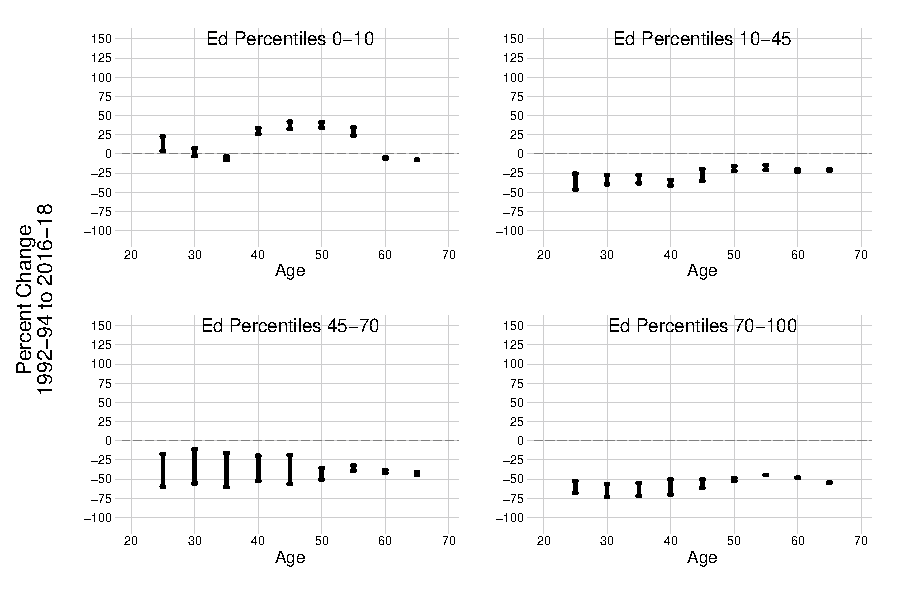
\includegraphics[scale=0.9]{\mortalitypath/changes-total-2-2} \\
      \panel{\textbf{D. Non-Hispanic Black Men}} \\
      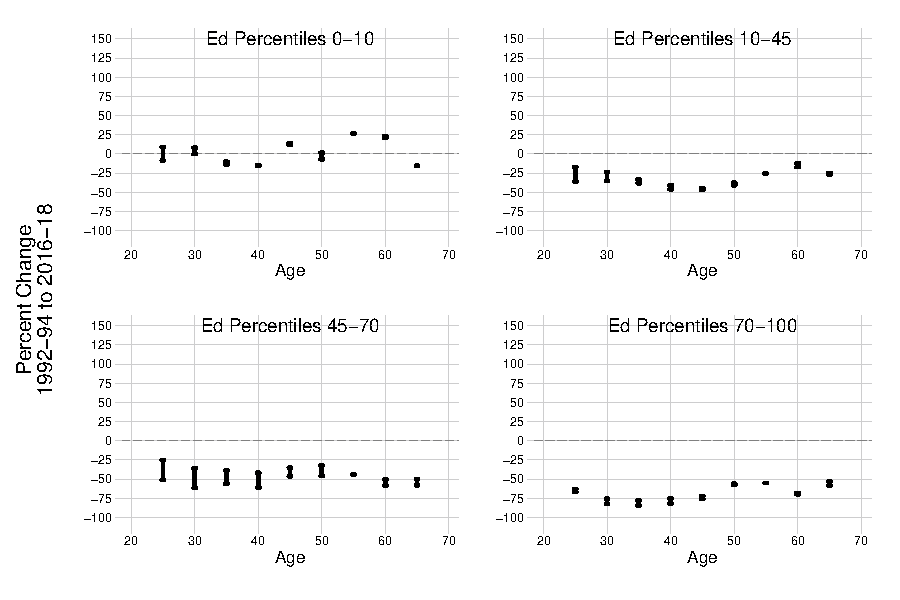
\includegraphics[scale=0.9]{\mortalitypath/changes-total-1-2} \\
    \end{tabular}
  \end{center}
  \vspace{-.5cm} \scriptsize{Note: The graph shows changes in
    mortality by age, sex, race, and constant percentile education bin. The vertical lines show the bounded set containing the percentage change in the mortality rate
    from 1992--1994 to 2016--2018 for the given age group. Bounds are
    computed using the set identification methods described in
    Section~\ref{sec:method}. Sources: ACS, CPS, NCHS.}
\end{figure}

%%%%%%%%%%%%%%%%%%%%%%%%%%%%%%%%%%%%%%%%%%%%%%%%%%%%%%%%%%%
%% FIGURE: CHANGES BY GROUP WITH ALL CAUSES OF MORTALITY %%
%%%%%%%%%%%%%%%%%%%%%%%%%%%%%%%%%%%%%%%%%%%%%%%%%%%%%%%%%%%
\begin{figure}[H]
  \caption{Decomposition of Mortality Change from 1992--94 to 2016--18: \cnewline
    Contribution of Deaths of Despair}
  \label{fig:mort_causes}

  \begin{center}
    \panel{\textbf{A. Non-Hispanic White Women}} \\
  \end{center}
  \begin{center}
    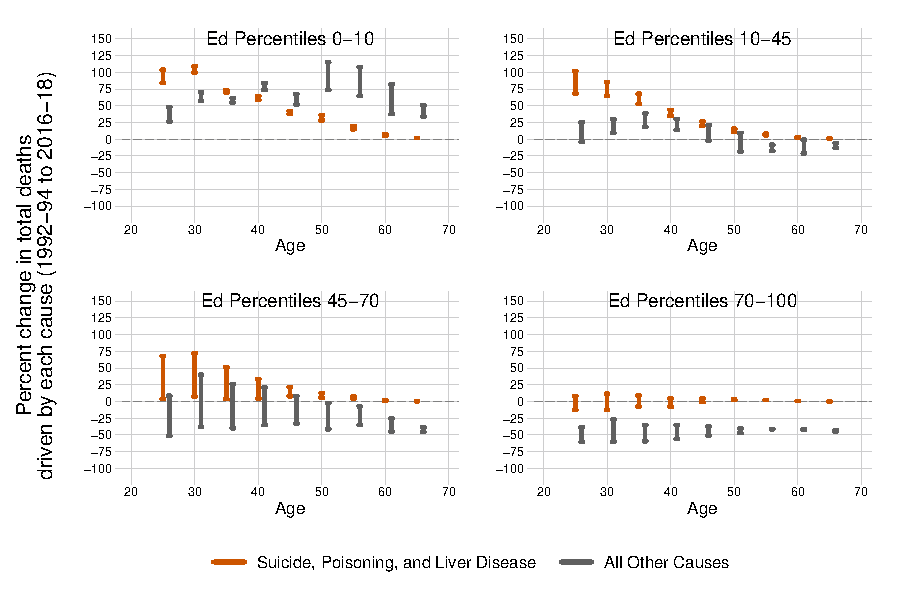
\includegraphics[scale=0.9]{\mortalitypath/changes-nod-2-1} &
  \end{center}

  \begin{center}
    \panel{\textbf{B. Non-Hispanic White Men}} \\
  \end{center}
  \begin{center}
    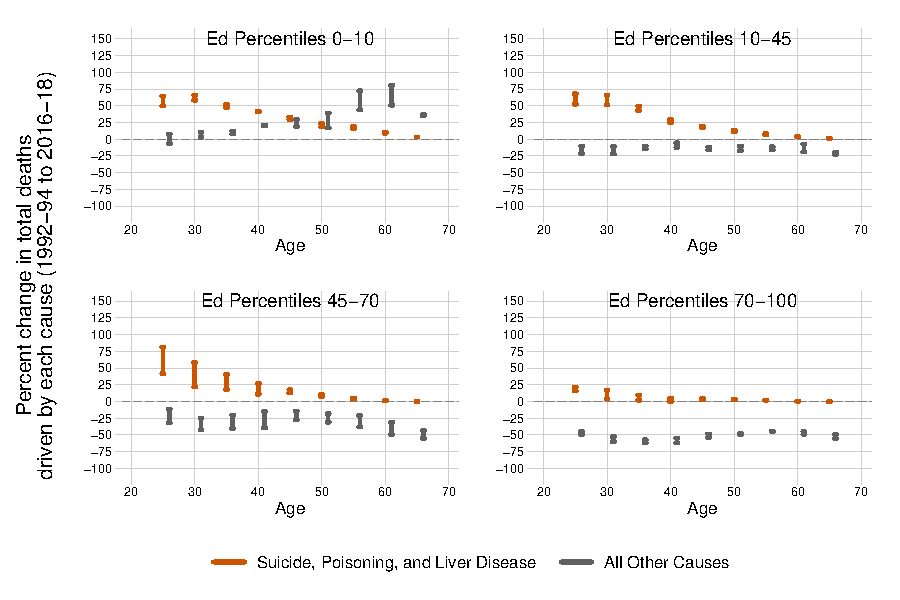
\includegraphics[scale=0.9]{\mortalitypath/changes-nod-1-1} \\
  \end{center}
\end{figure}
\begin{figure}[H]\ContinuedFloat

  \begin{center}
    \panel{\textbf{C. Non-Hispanic Black Women}} \\
  \end{center}
  \begin{center}
    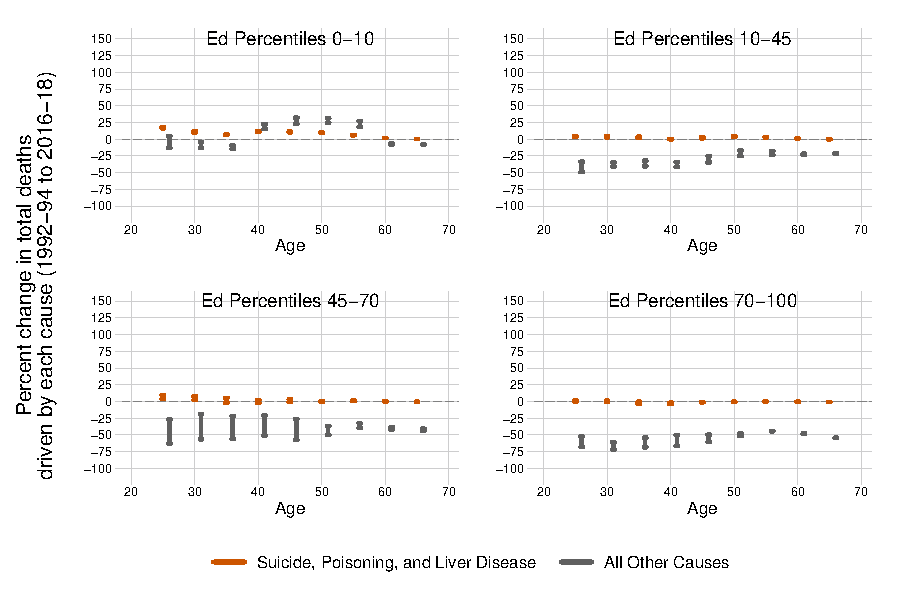
\includegraphics[scale=0.8]{\mortalitypath/changes-nod-2-2} &
  \end{center}
  \begin{center}
    \panel{\textbf{D. Non-Hispanic Black Men}} \\
  \end{center}
  \begin{center}
    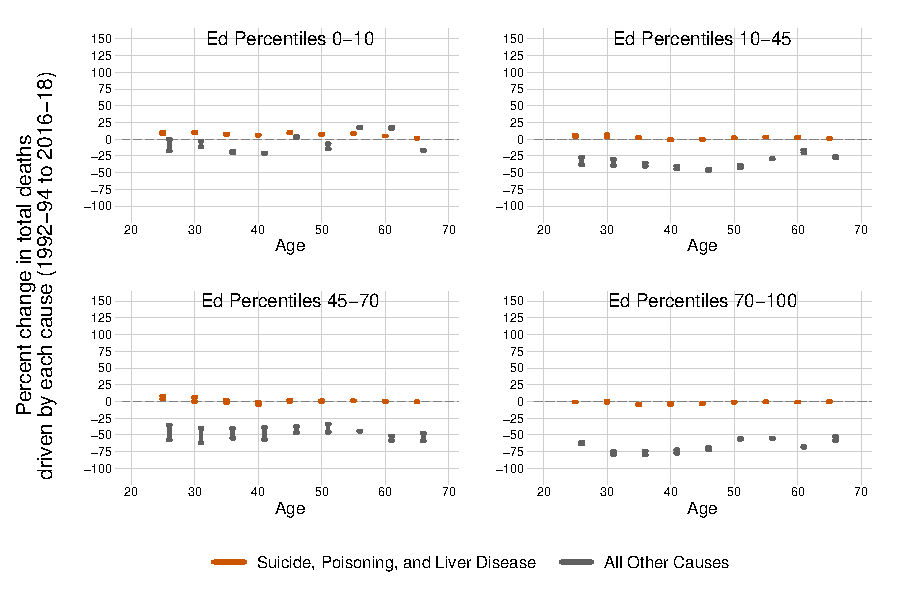
\includegraphics[scale=0.8]{\mortalitypath/changes-nod-1-2} \\
  \end{center}
\end{figure}
\vspace{-1cm}
\scriptsize{Note: ``White'' refers to non-Hispanic white. The graph decomposes the change in total mortality from 1992--1994 to 2016--2018 into two parts: the change in total deaths driven by deaths of despair, and the change in total deaths driven by all other causes. Estimates are disaggregated by age, sex, race, and constant percentile education bin. The orange lines show bounds on the contribution to total mortality change driven by changes in deaths of despair. The value on the $Y$ axis is the amount that total mortality for each group would have changed if the rates of all deaths \textit{other} than deaths of despair were unchanged. The gray lines show the contribution to total mortality change driven by all causes of death \textit{other} than deaths of despair. Deaths of despair are deaths from suicide, poisoning, and chronic liver disease. Bounds are computed using the set identification methods described in Section~\ref{sec:method}. Sources: ACS, CPS, NCHS.}
